\documentclass[11pt,oneside]{scrartcl}
\usepackage[a4paper,total={7in, 9.5in}]{geometry}

\newcommand{\mchname}{Mat\'{u}\v{s} Chochl\'{i}k}
\newcommand{\mchmail}{chochlik@gmail.com}
\newcommand{\docname}{Static reflection (revision 4)}
\newcommand{\docnum}{P0194R0}
\newcommand{\docdate}{2016-01-25}

\usepackage[utf8]{inputenc}
\usepackage{url}
\usepackage[colorlinks=true]{hyperref}
\usepackage{parskip}
\usepackage[titletoc]{appendix}

\usepackage{listings}
\usepackage{minted}
\lstset{basicstyle=\footnotesize\ttfamily,breaklines=true}

\usepackage{fancyhdr}
\setlength{\headheight}{14pt}
\pagestyle{fancyplain}
\lhead{\fancyplain{}{\docnum - \docname}}
\rhead{}
\rfoot{\fancyplain{}{\thepage}}
\cfoot{}

\usepackage[pdftex]{graphicx}
\DeclareGraphicsExtensions{.pdf}
\graphicspath{{images/}}
\usepackage{adjustbox}

\setcounter{tocdepth}{3} 

\title{\docname}

\author{\mchname (\mchmail)}

\newcommand{\concept}[1]{\hyperref[concept-#1]{\em{#1}}}
\newcommand{\meta}[1]{\concept{Meta#1}}

\begin{document}

\begin{tabular}{r l}
Document number: & \docnum\\
Date: & \docdate\\
Project: & Programming Language C++, SG7, Reflection\\
Reply-to: & \mchname (\href{mailto:\mchmail}{\mchmail})\\
\end{tabular}

\begin{center}
\vskip 2em
{\Huge \docname}
\vskip 1em
{\emph \mchname}
\vskip 2em
\end{center}

\paragraph{Abstract}

This paper is the follow-up to N3996, N4111 and N4451 and it is the fourth revision
of the proposal to add static reflection to the C++ standard.
It also introduces and briefly describes a partial, experimental implementation
of this proposal.

\tableofcontents

\section{Introduction}

Reflection and reflective programming can be used
for a wide range of tasks such as implementation of serialization-like operations,
remote procedure calls, scripting, automated GUI-generation,
implementation of several software design patterns, etc.
C++ as one of the most prevalent programming languages 
lacks a standardized reflection facility.

In this paper we propose the addition of native support for
compile-time reflection to C++ and a library built
on top of the metadata provided by the compiler.

The basic static metadata provided by compile-time reflection
should be as complete as possible to be applicable in a wide
range of scenarios and allow to implement custom higher-level
static and dynamic reflection libraries and reflection-based
utilities.

The term \emph{reflection} refers to the ability of a computer program
to observe and possibly alter its own structure and/or its behavior.
This includes building new or altering the existing data structures,
doing changes to algorithms or changing the way the program code
is interpreted. Reflective programming is a particular kind
of \emph{metaprogramming}.

The advantage of using reflection is in the fact that everything
is implemented in a single programming language, and the human-written
code can be closely tied with the customizable reflection-based
code which is automatically generated by compiler metaprograms,
based on the metadata provided by reflection.

The solution proposed in this paper is based on the
\href{http://kifri.fri.uniza.sk/~chochlik/mirror-lib/html/}{\em Mirror}
reflection utilities~\cite{mirror-doc-cpp11} and on several years
of user experience with reflection-based metaprogramming.

\section{Concept specification}
\label{section-current-Concepts}

We propose that the basic metadata describing a program written
in C++ should be made available through a set of {\em anonymous} types
defined by the compiler and through related functions and template classes.
At the moment these types should describe only the following program
declarations: namespaces\footnote{in a limited form}, types, typedefs,
classes and their data members and enum types.

In the future, the set of metaobjects should be extended to reflect
class inheritance, free functions, class member functions, templates,
template parameters, enumerated values, possibly the C++ specifiers, etc.

The compiler should generate metadata for the program declarations
in the currently processed translation unit, when requested by invoking
the reflection operator. Members of ordered sets (sequences) of metaobjects,
like scope members, parameters of a function, and so on, should be listed
in the order of appearance in the processed source code.

Since we want the metadata to be available at compile-time,
different base-level declarations should be reflected by
{\em statically different} metaobjects and thus by {\em different} types.
For example a metaobject reflecting the global scope namespace should
be a different {\em type} than a metaobject reflecting the \verb@std@
namespace\footnote{this means that they should be distinguishable for
example by the \texttt{std::is\_same} type trait},
a metaobject reflecting the \verb@int@ type should
have a different type then a metaobject reflecting the \verb@double@
type, etc.

This section describes\footnote{in pseudo-code} a set of metaobject concepts
and their requirements, traits for metaobject classification and operations
providing the individual bits of meta-data.

Unless stated otherwise, all proposed named templates described below should
go into the \verb@std::meta@ nested namespace in order to contain reflection-related
definitions and to help avoiding potential name conflicts.

\subsection{StringConstant}
\label{concept-StringConstant}

\texttt{StringConstant} represents a compile-time character string type. 

\begin{minted}[tabsize=4]{cpp}
struct StringConstant {
	typedef StringConstant type;
	typedef const char value_type[N+1];
	static constexpr const char value[N+1];

	operator const char* (void) const noexcept;
	const char* operator (void) const noexcept;
};
\end{minted}

This concept could be replaced by the \texttt{basic\_string\_constant}
from N4236.


\subsection{Meta-Object}
\label{concept-Meta-Object}

A \meta{Object} is a stateless anonymous type generated by the compiler
(when requested by the programmer through the 
\hyperref[section-reflection-operator]{\texttt{reflexpr} operator}),
providing metadata reflecting a specific program feature.

\subsubsection{\texttt{is\_metaobject}}

In order to distinguish between regular types and metaobjects generated
by the compiler, the \texttt{is\_metaobject} trait should be added
to the \texttt{std} namespace as one of the type traits. 

\begin{minted}{cpp}
template <typename T>
struct is_metaobject
{
	typedef bool value_type;
	static constexpr const bool value = /*
		true: if T is a metaobject
		false: otherwise
	*/

	typedef integral_constant<bool, value> type;

	operator value_type (void) const noexcept;
	value_type operator(void) const noexcept;
};

template <typename T>
using is_metaobject_t = typename is_metaobject<T>::type;

template <typename T>
constexpr bool is_metaobject_v = is_metaobject<T>::value;
\end{minted}

The expression \texttt{is\_metaobject<X>::value} should evaluate to \texttt{true}
if \texttt{X} is a metaobject generated by the compiler, otherwise it should
be \texttt{false}.

There are also several other trait templates nested in the namespace
\texttt{std::meta} which provide further information about metaobjects.
These traits are listed below together with their related metaobject concepts.



\subsubsection{Definition}

\begin{minted}{cpp}
namespace meta {
\end{minted}
\begin{minted}[xleftmargin=1em,tabsize=4,breakafter=&]{cpp}
template <typename T>
concept bool Object = is_metaobject_v<T>;

\end{minted}
\begin{minted}{cpp}
} // namespace meta
\end{minted}


The following operations are defined for each type satisfying the \meta{Object}
concept.



\subsubsection{\texttt{get\_source\_location}}

returns the source location info of the declaration of a base-level program feature reflected by a \meta{Object}.

\begin{minted}{cpp}
namespace meta {
\end{minted}
\begin{minted}[xleftmargin=1em,tabsize=4]{cpp}
template <Object T>
struct get_source_location : source_location { };

\end{minted}
\begin{minted}{cpp}
} // namespace meta
\end{minted}



The returned instance of \texttt{std::source\_location} should be \texttt{constexpr},
and the source file name and function name strings should be compile-time constants.

Also the source information for built-in types and other
such implicit declarations which are declared internally by the compiler
should return an empty string as a source file path and zero as source file
line and column.

\subsection{Meta-ObjectSequence}
\label{concept-Meta-ObjectSequence}

A \meta{ObjectSequence} is representing an ordered sequence of metaobjects.


\subsubsection{\texttt{is\_sequence}}

The \texttt{meta::is\_sequence}
trait indicates if the \meta{Object} passed as argument is a \meta{ObjectSequence}.

\input{sections/t_is_sequence_cpp.tex}


\subsubsection{Definition}

\begin{minted}{cpp}
namespace meta {
\end{minted}
\begin{minted}[xleftmargin=1em,tabsize=4,breakafter=&]{cpp}

template <typename T>
concept bool ObjectSequence = Object<T> && is_sequence_v<T>;

\end{minted}
\begin{minted}{cpp}
} // namespace meta
\end{minted}




\subsubsection{\texttt{get\_size}}

returns a number of elements in the sequence.

\begin{minted}{cpp}
namespace meta {
\end{minted}
\begin{minted}[xleftmargin=1em,tabsize=4]{cpp}
template <ObjectSequence T>
struct get_size : integral_constant<size_t, ...> { };
template <ObjectSequence T>
constexpr auto get_size_v = get_size<T>::value;
\end{minted}
\begin{minted}{cpp}
} // namespace meta
\end{minted}



\subsubsection{\texttt{get\_element}}

returns the i-th element in a ObjectSequence.

\begin{minted}{cpp}
namespace meta {
\end{minted}
\begin{minted}[xleftmargin=1em,tabsize=4]{cpp}
template <ObjectSequence T1, size_t Index>
struct get_element
{
	typedef /* generated by the compiler */ type;
};
	
template <ObjectSequence T1, size_t Index>
using get_element_t = typename get_element<T1, Index>::type;

\end{minted}
\begin{minted}{cpp}
} // namespace meta
\end{minted}


Note that \texttt{get\_element<...>::type}
must conform to the \meta{Object} concept.



\subsection{Meta-Named}
\label{concept-Meta-Named}

A \meta{Named} is a \meta{Declaration} reflecting a named base-level declaration
(namespace, type, variable, function, etc.).


\subsubsection{\texttt{has\_name}}

The \texttt{meta::has\_name}
trait indicates if the \meta{Declaration} passed as argument is a \meta{Named}.

\input{sections/t_has_name_cpp.tex}


\subsubsection{Definition}

\begin{minted}{cpp}
namespace meta {
\end{minted}
\begin{minted}[xleftmargin=1em,tabsize=4,breakafter=&]{cpp}

template <typename T>
concept bool Named = Object<T> && has_name_v<T>;

\end{minted}
\begin{minted}{cpp}
} // namespace meta
\end{minted}


\subsubsection{\texttt{get\_name}}

returns the basic name of the a named declaration reflected by a \meta{Named}.

\begin{minted}{cpp}
namespace meta {
\end{minted}
\begin{minted}[xleftmargin=1em,tabsize=4]{cpp}
template <Named T>
struct get_name : StringConstant { };
template <Named T>
constexpr auto get_name_v = get_name<T>::value;
\end{minted}
\begin{minted}{cpp}
} // namespace meta
\end{minted}


In case of types, the \texttt{get\_name} operation returns the type (or type alias)
name without any qualifiers, asterisks\footnote{in case of pointers},
ampersands\footnote{in case of references}, angle or square brackets\footnote{
in case of templates or arrays}, etc.

\subsection{Meta-Typed}
\label{concept-Meta-Typed}

A \meta{Typed} is a \meta{Declaration} reflecting base-level declaration with a type
(like a variable).


\subsubsection{\texttt{has\_type}}

The \texttt{meta::has\_type}
trait indicates if the \meta{Object} passed as argument is a \meta{Typed}.

\input{sections/t_has_type_cpp.tex}


\subsubsection{Definition}

\begin{minted}{cpp}
namespace meta {
\end{minted}
\begin{minted}[xleftmargin=1em,tabsize=4,breakafter=&]{cpp}

template <typename T>
concept bool Typed = Object<T> && has_type_v<T>;

\end{minted}
\begin{minted}{cpp}
} // namespace meta
\end{minted}



\subsubsection{\texttt{get\_type}}

returns the Type reflecting the type of base-level declaration with a type reflected by a \meta{Typed}.

\begin{minted}{cpp}
namespace meta {
\end{minted}
\begin{minted}[xleftmargin=1em,tabsize=4]{cpp}
template <Typed T>
struct get_type
{
	typedef /* generated by the compiler */ type;
};
	
template <Typed T>
using get_type_t = typename get_type<T>::type;

\end{minted}
\begin{minted}{cpp}
} // namespace meta
\end{minted}


Note that \texttt{get\_type<...>::type}
must conform to the \meta{Type} concept.


\subsection{Meta-Scoped}
\label{concept-Meta-Scoped}

A \meta{Scoped} is a \meta{Declaration} reflecting base-level declaration nested
inside of a scope.


\subsubsection{\texttt{has\_scope}}

The \texttt{meta::has\_scope}
trait indicates if the \meta{Declaration} passed as argument is a \meta{Scoped}.

\input{sections/t_has_scope_cpp.tex}


\subsubsection{Definition}

\begin{minted}{cpp}
namespace meta {
\end{minted}
\begin{minted}[xleftmargin=1em,tabsize=4,breakafter=&]{cpp}
template <Object T>
concept bool Scoped = has_scope_v<T>;

\end{minted}
\begin{minted}{cpp}
} // namespace meta
\end{minted}


\subsubsection{\texttt{get\_scope}}

returns the Scope reflecting the scope of a scoped declaration reflected by a \meta{Scoped}.

\begin{minted}[tabsize=4]{cpp}

template <typename T>
requires Scoped<T>
struct get_scope
{
	typedef Scope type;
};
	
template <typename T>
using get_scope_t = typename get_scope<T>::type;

\end{minted}


\subsection{Meta-Scope}
\label{concept-Meta-Scope}

A \meta{Scope} is a \meta{Object} which is usually also a \meta{Named}
and possibly a \meta{Scoped} reflecting a scope.


\subsubsection{\texttt{is\_scope}}

The \texttt{meta::is\_scope}
trait indicates if the \meta{Declaration} passed as argument is a \meta{Scope}.

\input{sections/t_is_scope_cpp.tex}


\subsubsection{Definition}

\begin{minted}{cpp}
namespace meta {
\end{minted}
\begin{minted}[xleftmargin=1em,tabsize=4,breakafter=&]{cpp}

template <typename T>
concept bool Scope = Object<T> && is_scope_v<T>;

\end{minted}
\begin{minted}{cpp}
} // namespace meta
\end{minted}


\subsection{Meta-Alias}
\label{concept-Meta-Alias}

A \meta{Alias} is a \meta{Named} reflecting a type or namespace alias.  


\subsubsection{\texttt{is\_alias}}

The \texttt{meta::is\_alias}
trait indicates if the \meta{Object} passed as argument is a \meta{Alias}.

\input{sections/t_is_alias_cpp.tex}


\subsubsection{Definition}

\begin{minted}{cpp}
namespace meta {
\end{minted}
\begin{minted}[xleftmargin=1em,tabsize=4,breakafter=&]{cpp}
template <Object T>
concept bool Alias = Named<T> && is_alias_v<T>;

\end{minted}
\begin{minted}{cpp}
} // namespace meta
\end{minted}


\subsubsection{\texttt{get\_aliased}}

returns the Named reflecting the original declaration of a type or namespace alias reflected by a \meta{Alias}.

\begin{minted}{cpp}
namespace meta {
\end{minted}
\begin{minted}[xleftmargin=1em,tabsize=4]{cpp}
template <Alias T>
struct get_aliased
{
	typedef /* generated by the compiler */ type;
	static_assert(Named<type>, "");
};
	
template <Alias T>
constexpr auto get_aliased_v = get_aliased<T>::value;
\end{minted}
\begin{minted}{cpp}
} // namespace meta
\end{minted}


\subsection{Meta-Linkable}
\label{concept-Meta-Linkable}

A \meta{Linkable} is a \meta{Named} and a \meta{Scoped} reflecting declaration with storage duration and/or linkage. 


\subsubsection{\texttt{is\_linkable}}

The \texttt{meta::is\_linkable}
trait indicates if the \meta{Declaration} passed as argument is a \meta{Linkable}.

\input{sections/t_is_linkable_cpp.tex}


\subsubsection{Definition}

\begin{minted}{cpp}
namespace meta {
\end{minted}
\begin{minted}[xleftmargin=1em,tabsize=4,breakafter=&]{cpp}

template <typename T>
concept bool Linkable = Named<T> && Scoped<T> && is_linkable_v<T>;

\end{minted}
\begin{minted}{cpp}
} // namespace meta
\end{minted}



\subsubsection{\texttt{is\_static}}

returns whether the declaration with storage duration and/or linkage reflected by a \meta{Linkable} was declared with the static specifier.

\begin{minted}{cpp}
namespace meta {
\end{minted}
\begin{minted}[xleftmargin=1em,tabsize=4]{cpp}
template <Linkable T>
struct is_static : integral_constant<bool, ...> { };
template <Linkable T>
constexpr auto is_static_v = is_static<T>::value;
\end{minted}
\begin{minted}{cpp}
} // namespace meta
\end{minted}



\subsection{Meta-ClassMember}
\label{concept-Meta-ClassMember}

A \meta{ClassMember} is a \meta{Scoped} reflecting a class member.


\subsubsection{\texttt{is\_class\_member}}

The \texttt{meta::is\_class\_member}
trait indicates if the \meta{Declaration} passed as argument is a \meta{ClassMember}.

\input{sections/t_is_class_member_cpp.tex}


\subsubsection{Definition}

\begin{minted}{cpp}
namespace meta {
\end{minted}
\begin{minted}[xleftmargin=1em,tabsize=4,breakafter=&]{cpp}

template <typename T>
concept bool ClassMember = Scoped<T> && is_class_member_v<T> && is_class_v<get_scope_t<T>>;

\end{minted}
\begin{minted}{cpp}
} // namespace meta
\end{minted}


\subsubsection{\texttt{is\_public}}

returns whether the class member reflected by a \meta{ClassMember} was declared with public access.

\begin{minted}[tabsize=4]{cpp}

template <typename T>
requires ClassMember<T>
struct is_public : integral_constant<bool, ...> { };
template <typename T>
using is_public_t = typename is_public<T>::type;

\end{minted}



\subsection{Meta-GlobalScope}
\label{concept-Meta-GlobalScope}

A \meta{GlobalScope} is a \meta{Scope} reflecting the global scope.


\subsubsection{\texttt{is\_global\_scope}}

The \texttt{meta::is\_global\_scope}
trait indicates if the \meta{Declaration} passed as argument is a \meta{GlobalScope}.

\input{sections/t_is_global_scope_cpp.tex}


\subsubsection{Definition}

\begin{minted}[tabsize=8]{cpp}
namespace meta {

template <typename T>
concept bool GlobalScope =
	Scope<T> &&
	meta::is_global_scope_v<T>;

} // namespace meta
\end{minted}


\subsection{Meta-Namespace}
\label{concept-Meta-Namespace}

A \meta{Namespace} is a \meta{Named}, a \meta{Scoped} and a \meta{Scope}
reflecting a namespace.


\subsubsection{\texttt{is\_namespace}}

The \texttt{meta::is\_namespace}
trait indicates if the \meta{Declaration} passed as argument is a \meta{Namespace}.

\input{sections/t_is_namespace_cpp.tex}


\subsubsection{Definition}

\begin{minted}{cpp}
namespace meta {
\end{minted}
\begin{minted}[xleftmargin=1em,tabsize=4,breakafter=&]{cpp}
template <Object T>
concept bool Namespace = Named<T> && Scope<T> && Scoped<T> && is_namespace_v<T>;

\end{minted}
\begin{minted}{cpp}
} // namespace meta
\end{minted}


\subsection{Meta-NamespaceAlias}
\label{concept-Meta-NamespaceAlias}

A \meta{NamespaceAlias} is a \meta{Namespace} and a \meta{Alias}
reflecting a namespace alias.


\subsubsection{Definition}

\begin{minted}[tabsize=8]{cpp}
namespace meta {

template <typename T>
concept bool NamespaceAlias =
	Namespace<T> &&
	Alias<T> &&
	meta::is_namespace_v<get_aliased_t<T>>;

} // namespace meta
\end{minted}



\subsection{Meta-Type}
\label{concept-Meta-Type}

A \meta{Type} is a \meta{Named} and a \meta{Scoped}
reflecting a type.


\subsubsection{\texttt{is\_type}}

The \texttt{meta::is\_type}
trait indicates if the \meta{Object} passed as argument is a \meta{Type}.

\input{sections/t_is_type_cpp.tex}


\subsubsection{Definition}

\begin{minted}[tabsize=8]{cpp}
namespace meta {

template <typename T>
concept bool Type =
	Named<T> &&
	Scoped<T> &&
	meta::is_type_v<T>;

} // namespace meta
\end{minted}



\subsubsection{\texttt{get\_reflected\_type}}

returns the the base-level type reflected by a \meta{Type}.

\begin{minted}{cpp}
namespace meta {
\end{minted}
\begin{minted}[xleftmargin=1em,tabsize=4]{cpp}
template <Type T>
struct get_reflected_type
{
	typedef /* generated by the compiler */ type;
};
	
template <Type T>
constexpr auto get_reflected_type_v = get_reflected_type<T>::value;
\end{minted}
\begin{minted}{cpp}
} // namespace meta
\end{minted}



\subsection{Meta-TypeAlias}
\label{concept-Meta-TypeAlias}

A \meta{TypeAlias} is a \meta{Type} and a \meta{Alias}
reflecting a typedef, a type alias or a substituted template type parameter.


\subsubsection{Definition}

\begin{minted}{cpp}
namespace meta {
\end{minted}
\begin{minted}[xleftmargin=1em,tabsize=4,breakafter=&]{cpp}

template <typename T>
concept bool TypeAlias = Type<T> && Alias<T> && is_type_v<get_aliased_t<T>>;

\end{minted}
\begin{minted}{cpp}
} // namespace meta
\end{minted}


If the reflected type alias or typedef refers to a class then the reflecting
\meta{TypeAlias} is also a \meta{Class}, if the reflected alias refers
to an enum then the \meta{TypeAlias} is also a \meta{Enum}.

\subsection{Meta-Class}
\label{concept-Meta-Class}

A \meta{Class} is a \meta{Type} and a \meta{Scope}
reflecting a class, struct or union.


\subsubsection{\texttt{is\_class}}

The \texttt{meta::is\_class}
trait indicates if the \meta{Object} passed as argument is a \meta{Class}.

\input{sections/t_is_class_cpp.tex}


\subsubsection{Definition}

\begin{minted}{cpp}
namespace meta {
\end{minted}
\begin{minted}[xleftmargin=1em,tabsize=4,breakafter=&]{cpp}

template <typename T>
concept bool Class = Type<T> && Scope<T> && is_class_v<T>;

\end{minted}
\begin{minted}{cpp}
} // namespace meta
\end{minted}


\subsubsection{\texttt{get\_data\_members}}

returns a sequence of objects reflecting the public data members of a class reflected by a \meta{Class}.

\begin{minted}[tabsize=4]{cpp}

template <typename T>
requires Class<T>
struct get_data_members
{
	typedef DeclarationSequence type;
};
	
template <typename T>
using get_data_members_t = typename get_data_members<T>::type;

\end{minted}

\subsubsection{\texttt{get\_all\_data\_members}}

returns a sequence of objects reflecting all    (including the private and protected)   data members of a class reflected by a \meta{Class}.

\begin{minted}[tabsize=4]{cpp}

template <typename T>
requires Class<T>
struct get_all_data_members
{
	typedef DeclarationSequence type;
};
	
template <typename T>
using get_all_data_members_t = typename get_all_data_members<T>::type;

\end{minted}


The \meta{DeclarationSequence} returned by \texttt{get\_data\_members} and
\texttt{get\_all\_data\_members} should \emph{not} include metaobjects reflecting
inherited data members.

\subsection{Meta-Enum}
\label{concept-Meta-Enum}

A \meta{Enum} is a \meta{Type} and possibly also a \meta{Scope}
reflecting an enum or a scoped enum.


\subsubsection{\texttt{is\_enum}}

The \texttt{meta::is\_enum}
trait indicates if the \meta{Object} passed as argument is a \meta{Enum}.

\input{sections/t_is_enum_cpp.tex}


\subsubsection{Definition}

\begin{minted}{cpp}
namespace meta {
\end{minted}
\begin{minted}[xleftmargin=1em,tabsize=4,breakafter=&]{cpp}

template <typename T>
concept bool Enum = Type<T> && is_enum_v<T>;

\end{minted}
\begin{minted}{cpp}
} // namespace meta
\end{minted}


\subsection{Meta-EnumClass}
\label{concept-Meta-EnumClass}

A \meta{EnumClass} is a \meta{Enum} and a \meta{Scope}
reflecting a scoped, strongly-typed enumeration.


\subsubsection{Definition}

\begin{minted}[tabsize=8]{cpp}
namespace meta {

template <typename T>
concept bool EnumClass =
	Enum<T> &&
	Scope<T>;

} // namespace meta
\end{minted}


\subsection{Meta-Variable}
\label{concept-Meta-Variable}

A \meta{Variable} is a \meta{Named}, a \meta{Typed} and a \meta{Linkable}
reflecting a variable\footnote{At the moment only class data members fall
into this category, but variable reflection should be introduced in a future
proposal}.


\subsubsection{\texttt{is\_variable}}

The \texttt{meta::is\_variable}
trait indicates if the \meta{Declaration} passed as argument is a \meta{Variable}.

\input{sections/t_is_variable_cpp.tex}


\subsubsection{Definition}

\begin{minted}{cpp}
namespace meta {
\end{minted}
\begin{minted}[xleftmargin=1em,tabsize=4,breakafter=&]{cpp}

template <typename T>
concept bool Variable = Named<T> && Typed<T> && Linkable<T> && is_variable_v<T>;

\end{minted}
\begin{minted}{cpp}
} // namespace meta
\end{minted}


\subsubsection{\texttt{get\_pointer}}

returns a pointer to the a variable reflected by a \meta{Variable}.   If the variable is a class member then the pointer is a class data member pointer,   otherwise it is a plain pointer.

\begin{minted}[tabsize=4]{cpp}

template <typename T>
requires Variable<T>
struct get_pointer
{
	typedef conditional_t<
		is_class_member_v<T> && !is_static_v<T>,
		get_reflected_type_t<get_type_t<T>>
		get_reflected_type_t<get_scope_t<T>>::*,
		get_reflected_type_t<get_type_t<T>>*
	> value_type;

	static const value_type value;
};
	
template <typename T>
const auto get_pointer_v = get_pointer<T>::value;

\end{minted}


\subsection{Meta-DataMember}
\label{concept-Meta-DataMember}

A \meta{DataMember} is a \meta{Variable} and a \meta{ClassMember}
reflecting a class data member.


\subsubsection{Definition}

\begin{minted}[tabsize=8]{cpp}
namespace meta {

template <typename T>
concept bool DataMember =
	Variable<T> &&
	ClassMember<T>;

} // namespace meta
\end{minted}



\section{Reflection operator}

The metaobjects reflecting some program feature \verb@X@ as
described above should be made available to the user by
the means of a new operator or expression.
More precisely, the reflection operator should return a type conforming to a particular
metaobject concept, depending on the reflected expression.

Since adding a new keyword has the potential to break existing code,
we do not insist on any particular expression, here follows a list of suggestions
in order of preference (from the most to the least preferrable):

\begin{itemize}
\item{\verb@mirrored(X)@}
\item{\verb@reflected(X)@}
\item{\verb@reflexpr(X)@}
\item{\verb@|X@}
\item{\verb@[[X]]@}
\item{\verb@<<X>>@}
\end{itemize}

The reflected expression \verb@X@ in the items listed above can be any of the following:

\begin{itemize}
\item{\verb@::@} -- The global scope, the returned metaobject is a {\meta{GlobalScope}}.
\item{{\em Namespace name}} -- (\verb@std@) the returned metaobject is a {\meta{Namespace}}.
\item{{\em Type name}} -- (\verb@long double@) the returned metaobject is a {\meta{Type}}.
\item{{\em \verb@typedef@ name}} -- (\verb@std::size_t@ or \verb@std::string@)
     the returned metaobject is a {\meta{Typedef}}.
\item{{\em Template name}} -- (\verb@std::tuple@ or \verb@std::map@)
     the returned metaobject is a {\meta{Template}}.
\item{{\em Class name}} -- (\verb@std::thread@ or \verb@std::map<int, double>@)
     the returned metaobject is a {\meta{Class}}.
\item{{\em Function name}} -- (\verb@std::sin@ or \verb@std::string::size@) the returned metaobject
     is a {\meta{OverloadedFunction}}.
\item{{\em Function signature}} -- (\verb@std::sin(double)@ or \verb@std::string::front(void) const@)
     the returned metaobject is a {\meta{Function}}. The signature may be specified without the
     return value type.
\item{{\em Constructor signature}} -- (\verb@std::pair<char, double>::pair(char, double)@
     or \verb@std::string::string(void)@) the returned metaobject is a {\meta{Constructor}}.
\item{{\em Variable name}} -- (\verb@std::errno@) the returned metaobject is a {\meta{Variable}}.
%\item{TODO}
\end{itemize}

The reflection operator or expression should have access to \verb@private@ and
\verb@protected@ members of classes. The following should be valid:

\begin{minted}{cpp}
struct A
{
	int a;
};

class B
{
protected:
	int b;
};

class C
 : protected A
 , public B
{
private:
	int c;
};

typedef mirrored(A::a) meta_A_a;
typedef mirrored(B::b) meta_B_b;
typedef mirrored(C::a) meta_C_a;
typedef mirrored(C::b) meta_C_b;
typedef mirrored(C::c) meta_C_c;

\end{minted}

\subsection{Context-dependent reflection}

We also propose to define a set of special expressions that can be used
inside of the reflection operator, to obtain metadata based on the context
where it is invoked, instead of the identifier.

\subsubsection{Namespaces}

If the \verb@this::namespace@ expression is used as the argument of the reflection
operator, then it should return a \meta{Namespace} reflecting the namespace
inside of which the reflection operator was invoked.

For example:

\begin{minted}{cpp}

typedef mirrored(this::namespace) _meta_gs;

\end{minted}

reflects the global scope namespace and is equivalent to

\begin{minted}{cpp}

typedef mirrored(::) _meta_gs;

\end{minted}

For named namespaces:

\begin{minted}{cpp}

namespace foo {

typedef mirrored(this::namespace) _meta_foo;

namespace bar {

typedef mirrored(this::namespace) _meta_foo_bar;

} // namespace bar

} // namespace foo
\end{minted}

\subsubsection{Classes}

If the \verb@this::class@ expression is used as the argument of the reflection
operator, then it should return a \meta{Class} reflecting the class
inside of which the reflection operator was invoked.

For example:

\begin{minted}{cpp}

struct foo
{
	const char* _name;

	// reflects foo
	typedef mirrored(this::class) _meta_foo1;

	foo(void)
	 : _name(base_name<mirrored(this::class)>())
	{ }

	void f(void)
	{
		// reflects foo
		typedef mirrored(this::class) _meta_foo2;
	}

	double g(double, double);

	struct bar
	{
		// reflects foo::bar
		typedef mirrored(this::class) _meta_foo_bar;
	};
};

double foo::g(double a, double b)
{
	// reflects foo
	typedef mirrored(this::class) _meta_foo3;
	return a+b;
}

class baz
{
private:
	typedef mirrored(this::class) _meta_baz;
};

typedef mirrored(this::class); // <- error: not used inside of a class.

\end{minted}

\subsubsection{Functions}

If the \verb@this::function@ expression is used as the argument of the reflection
operator, then it should return a \meta{Function} reflecting the function or operator
inside of which the reflection operator was invoked.

For example:

\begin{minted}{cpp}

void foobar(void)
{
	// reflects this particular overload of the foobar function
	typedef mirrored(this::function) _meta_foobar;
}

int foobar(int i)
{
	// reflects this particular overload of the foobar function
	typedef mirrored(this::function) _meta_foobar;
	return i+1;
}

class foo
{
private:
	void f(void)
	{
		// reflects this particular overload of foo::f
		typedef mirrored(this::function) _meta_foo_f;
	}

	double f(void)
	{
		// reflects this particular overload of foo::f
		typedef mirrored(this::function) _meta_foo_f;
		return 12345.6789;
	}
public:
	foo(void)
	{
		// reflects this constructor of foo
		typedef mirrored(this::function) _meta_foo_foo;
	}

	friend bool operator == (foo, foo)
	{
		// reflects this operator
		typedef mirrored(this::function) _meta_foo_eq;
	}

	typedef mirrored(this::function) _meta_fn; // <- error
};

typedef mirrored(this::function) _meta_fn; // <- error

\end{minted}


\section{Experimental implementation}

A fork of the clang compiler with a partial experimental implementation
of this proposal can be found on github \cite{clang-reflexpr-impl}.
The modified compiler can be built by following the instructions listed
in \cite{clang-getting-started}, but instead of checking out the official clang
repository, the sources on the \texttt{mirror-reflection} branch of the modified
repository should be used.

The implementation required changes (mostly additions) to roughly 3500 lines
of code in the compiler plus circa 540 lines in the \texttt{<reflexpr>} header.

All examples listed in Appendix \ref{section-reflexpr-examples} are working with
the modified compiler.

This particular implementation works by generating and adding new \texttt{CXXRecordDecl}s,
with member typedefs and member constants providing basic meta-data, to the AST.
The templates implementing the metaobject operations are referencing and
occasionally transforming the members of the metaobject types.

The \texttt{is\_metaobject} trait is implemented by extending the existing
clang's type-trait framework and adding the \texttt{\_\_is\_metaobject} builtin
operator.

The \meta{DeclarationSequence} operations, namely \texttt{get\_size} and
\texttt{get\_element} are implemented lazily by using the new
\texttt{\_\_reflexpr\_size} and \texttt{\_\_reflexpr\_element} operators.



\renewcommand\refname{\arabic{section}\hspace{1em}References}

\stepcounter{section}
\addcontentsline{toc}{section}{\refname}

\begin{thebibliography}{100}

\bibitem{mirror-doc-cpp11}
Mirror C++ reflection library documentation (C++11 version),
\url{http://kifri.fri.uniza.sk/~chochlik/mirror-lib/html/}.

\end{thebibliography}{100}



\begin{appendices}
\newpage
\appendix
\part*{Appendix}
\addcontentsline{toc}{part}{Appendix}
\section{Diagrams}

\begin{figure}[H]
\centering
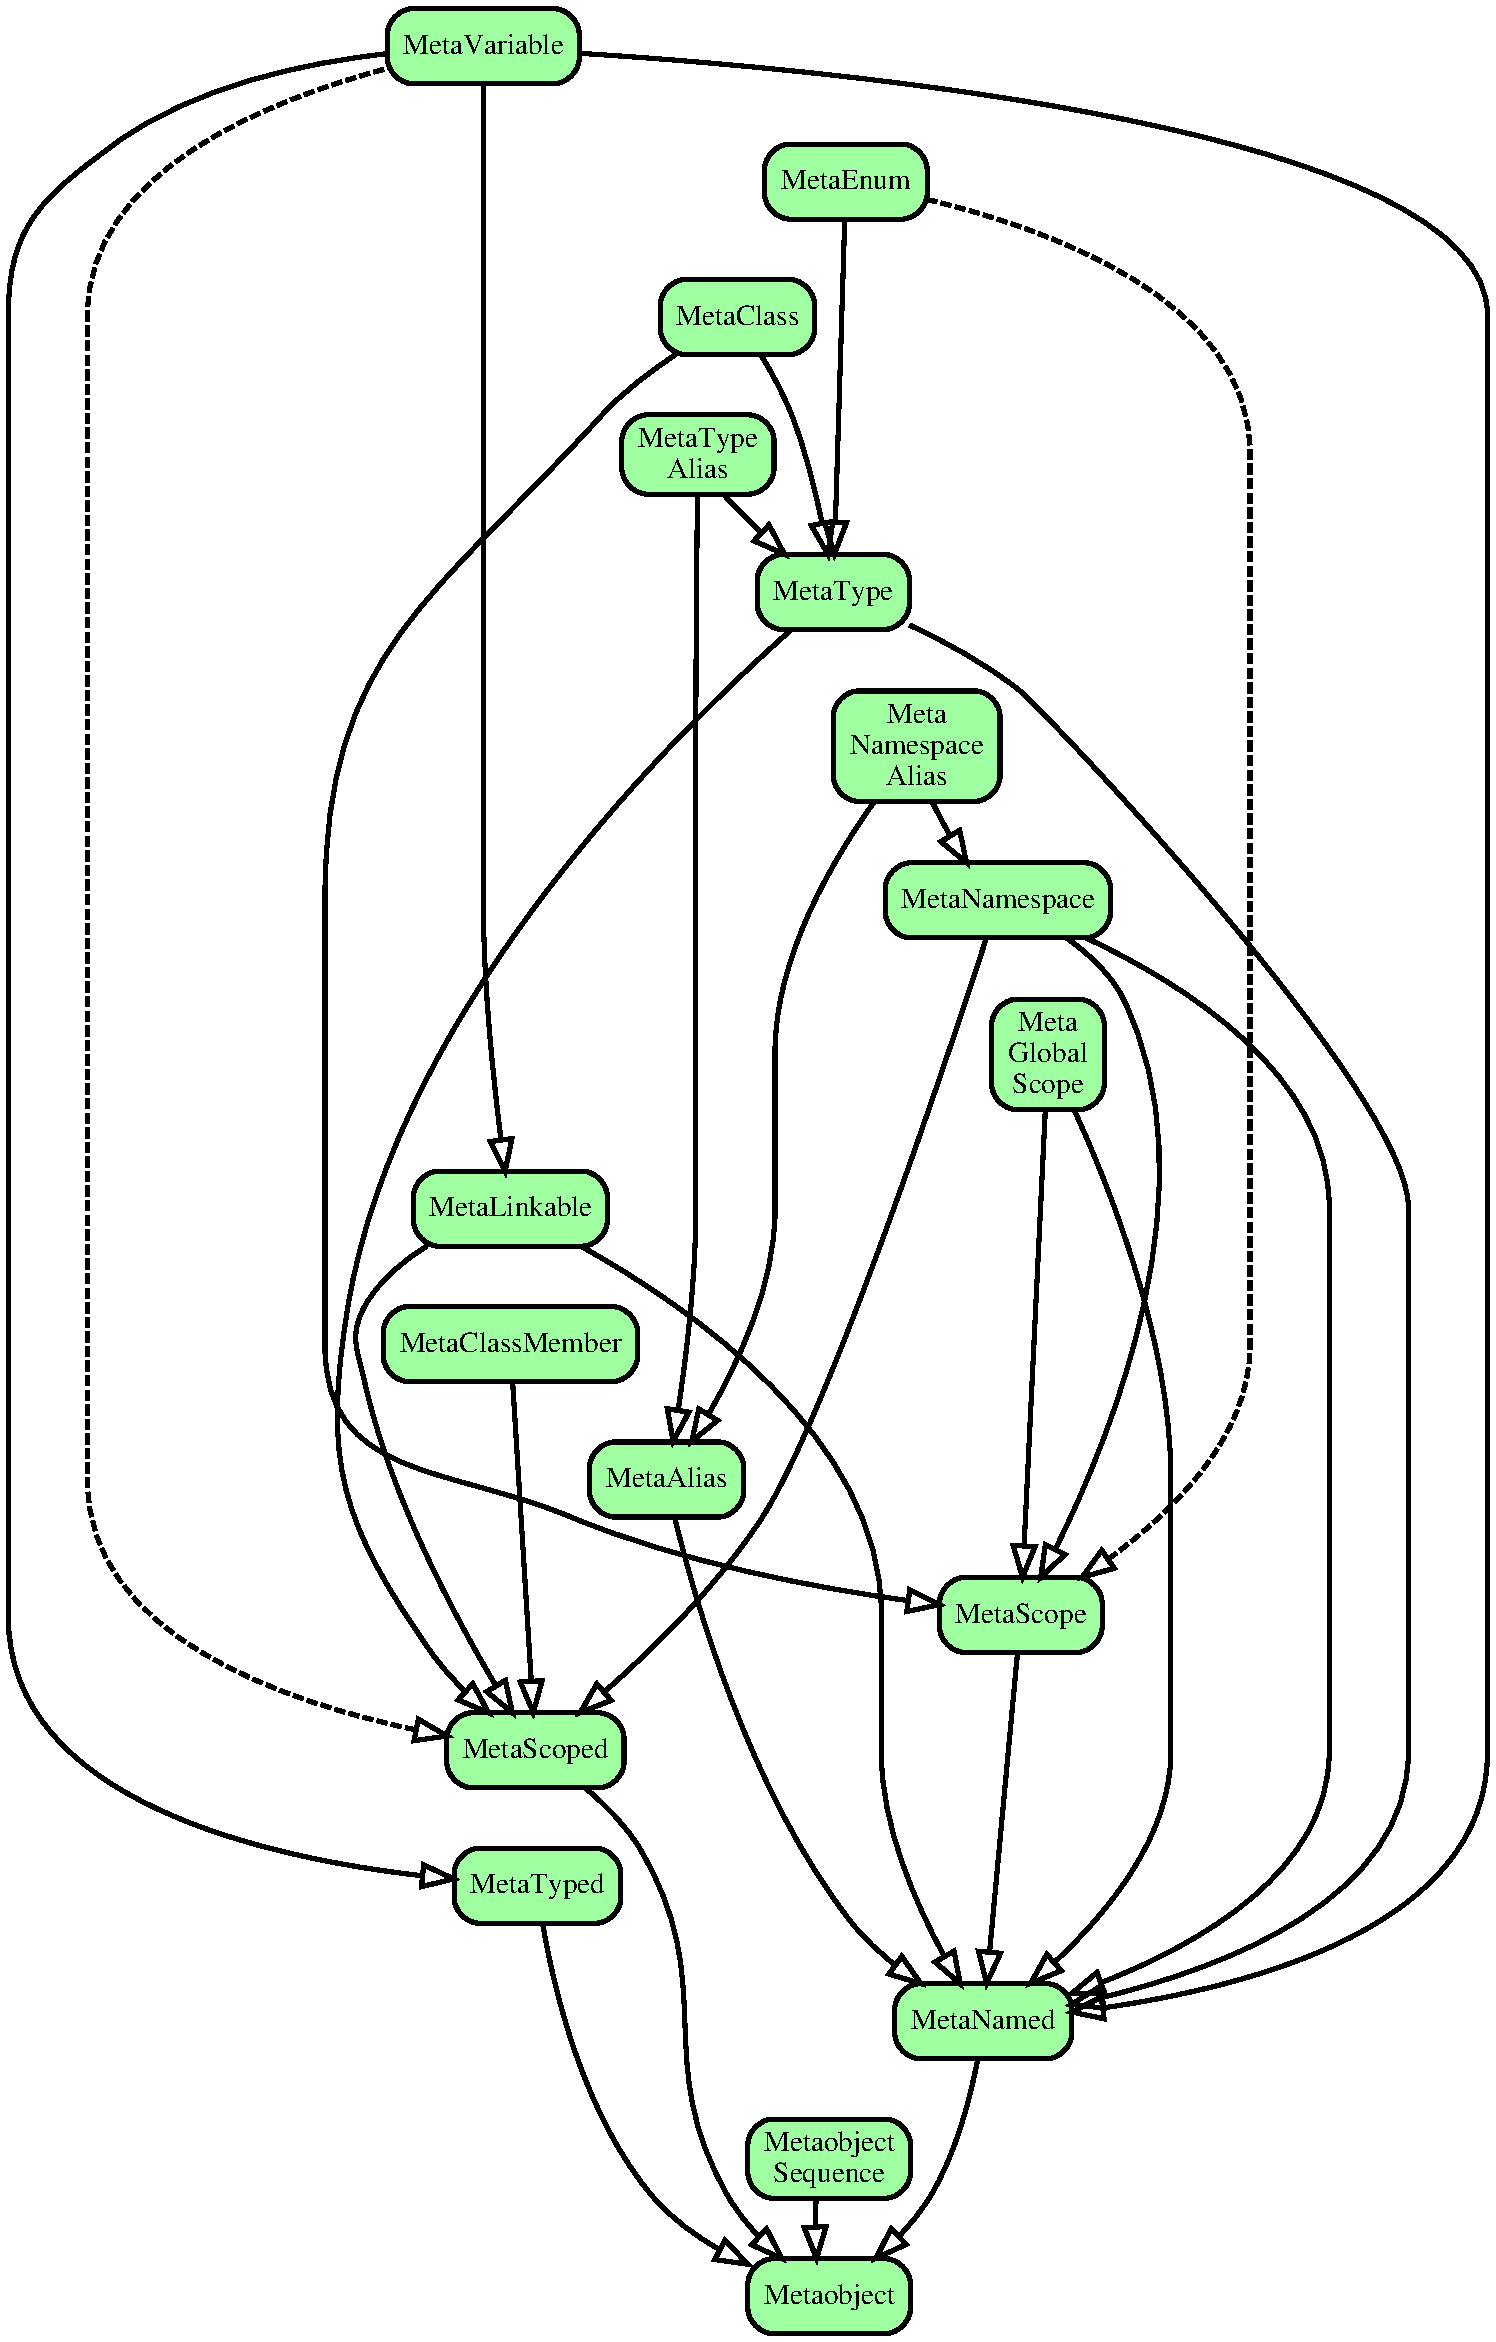
\includegraphics[height=0.8\textheight]{hierarchy.pdf}
\caption{Metaobject concept inheritance hierarchy}
\end{figure}

\begin{figure}[H]
\centering
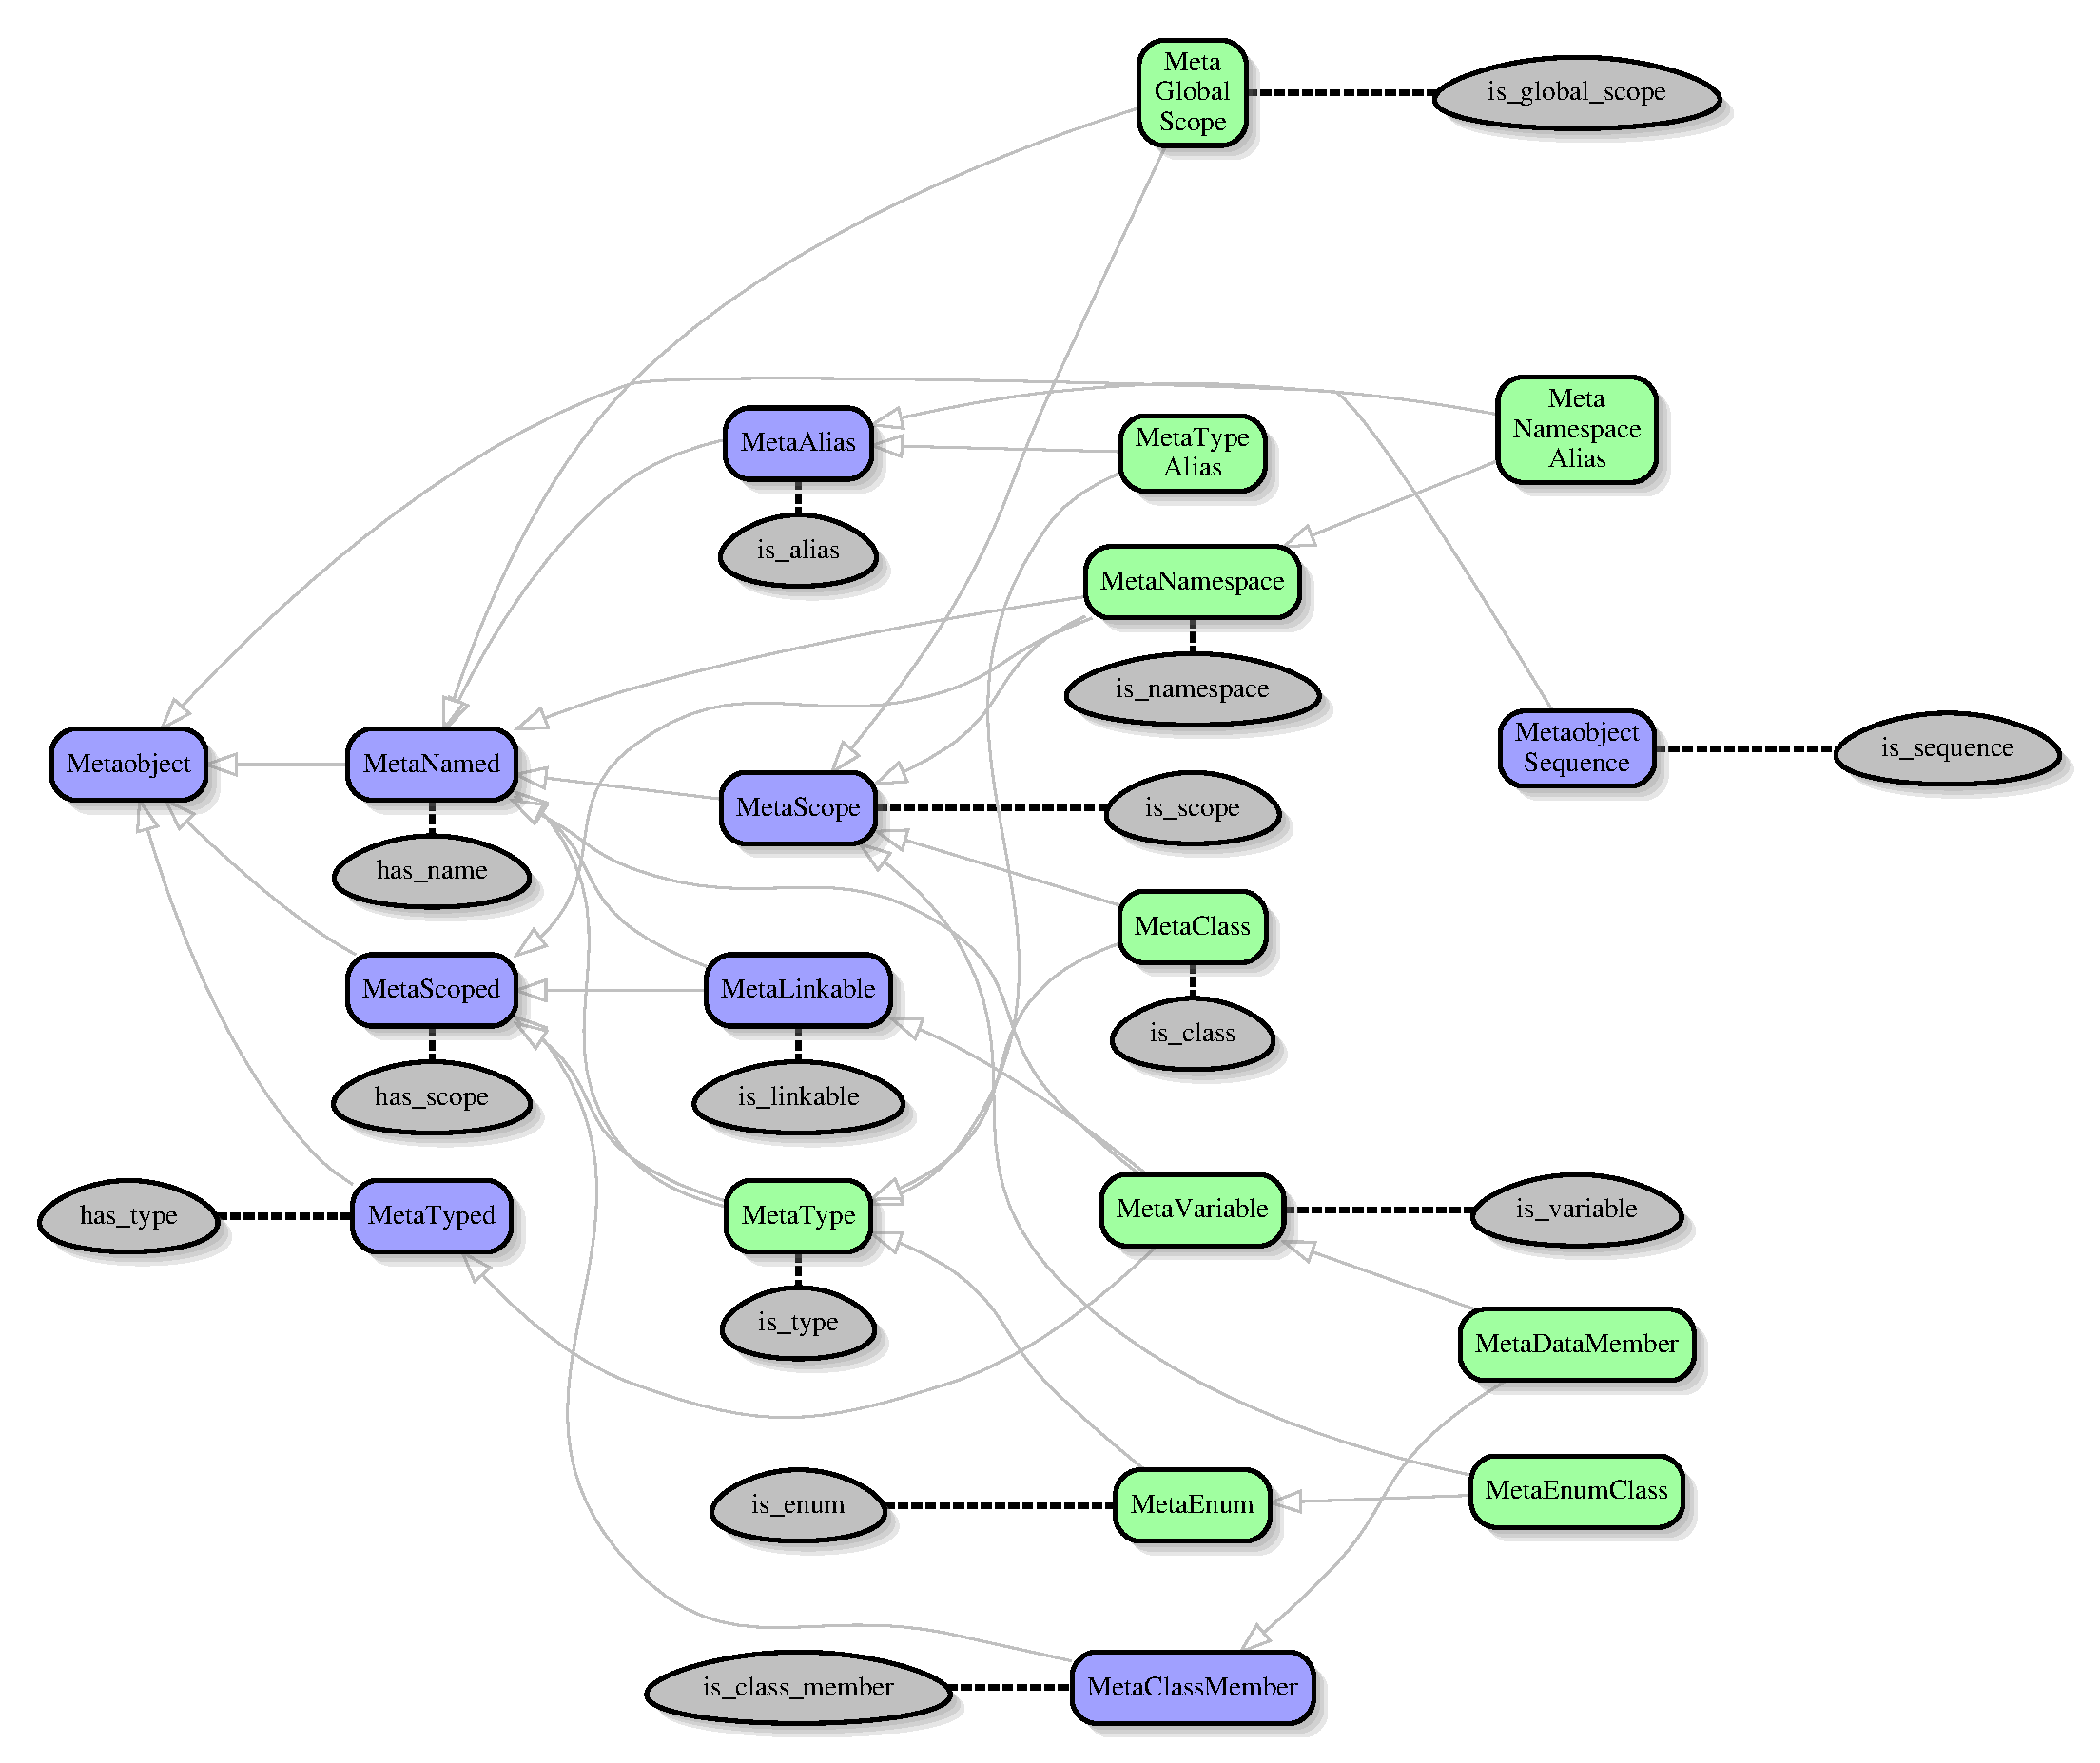
\includegraphics[width=\textwidth]{traits.pdf}
\caption{Metaobject traits}
\end{figure}

\begin{figure}[H]
\centering
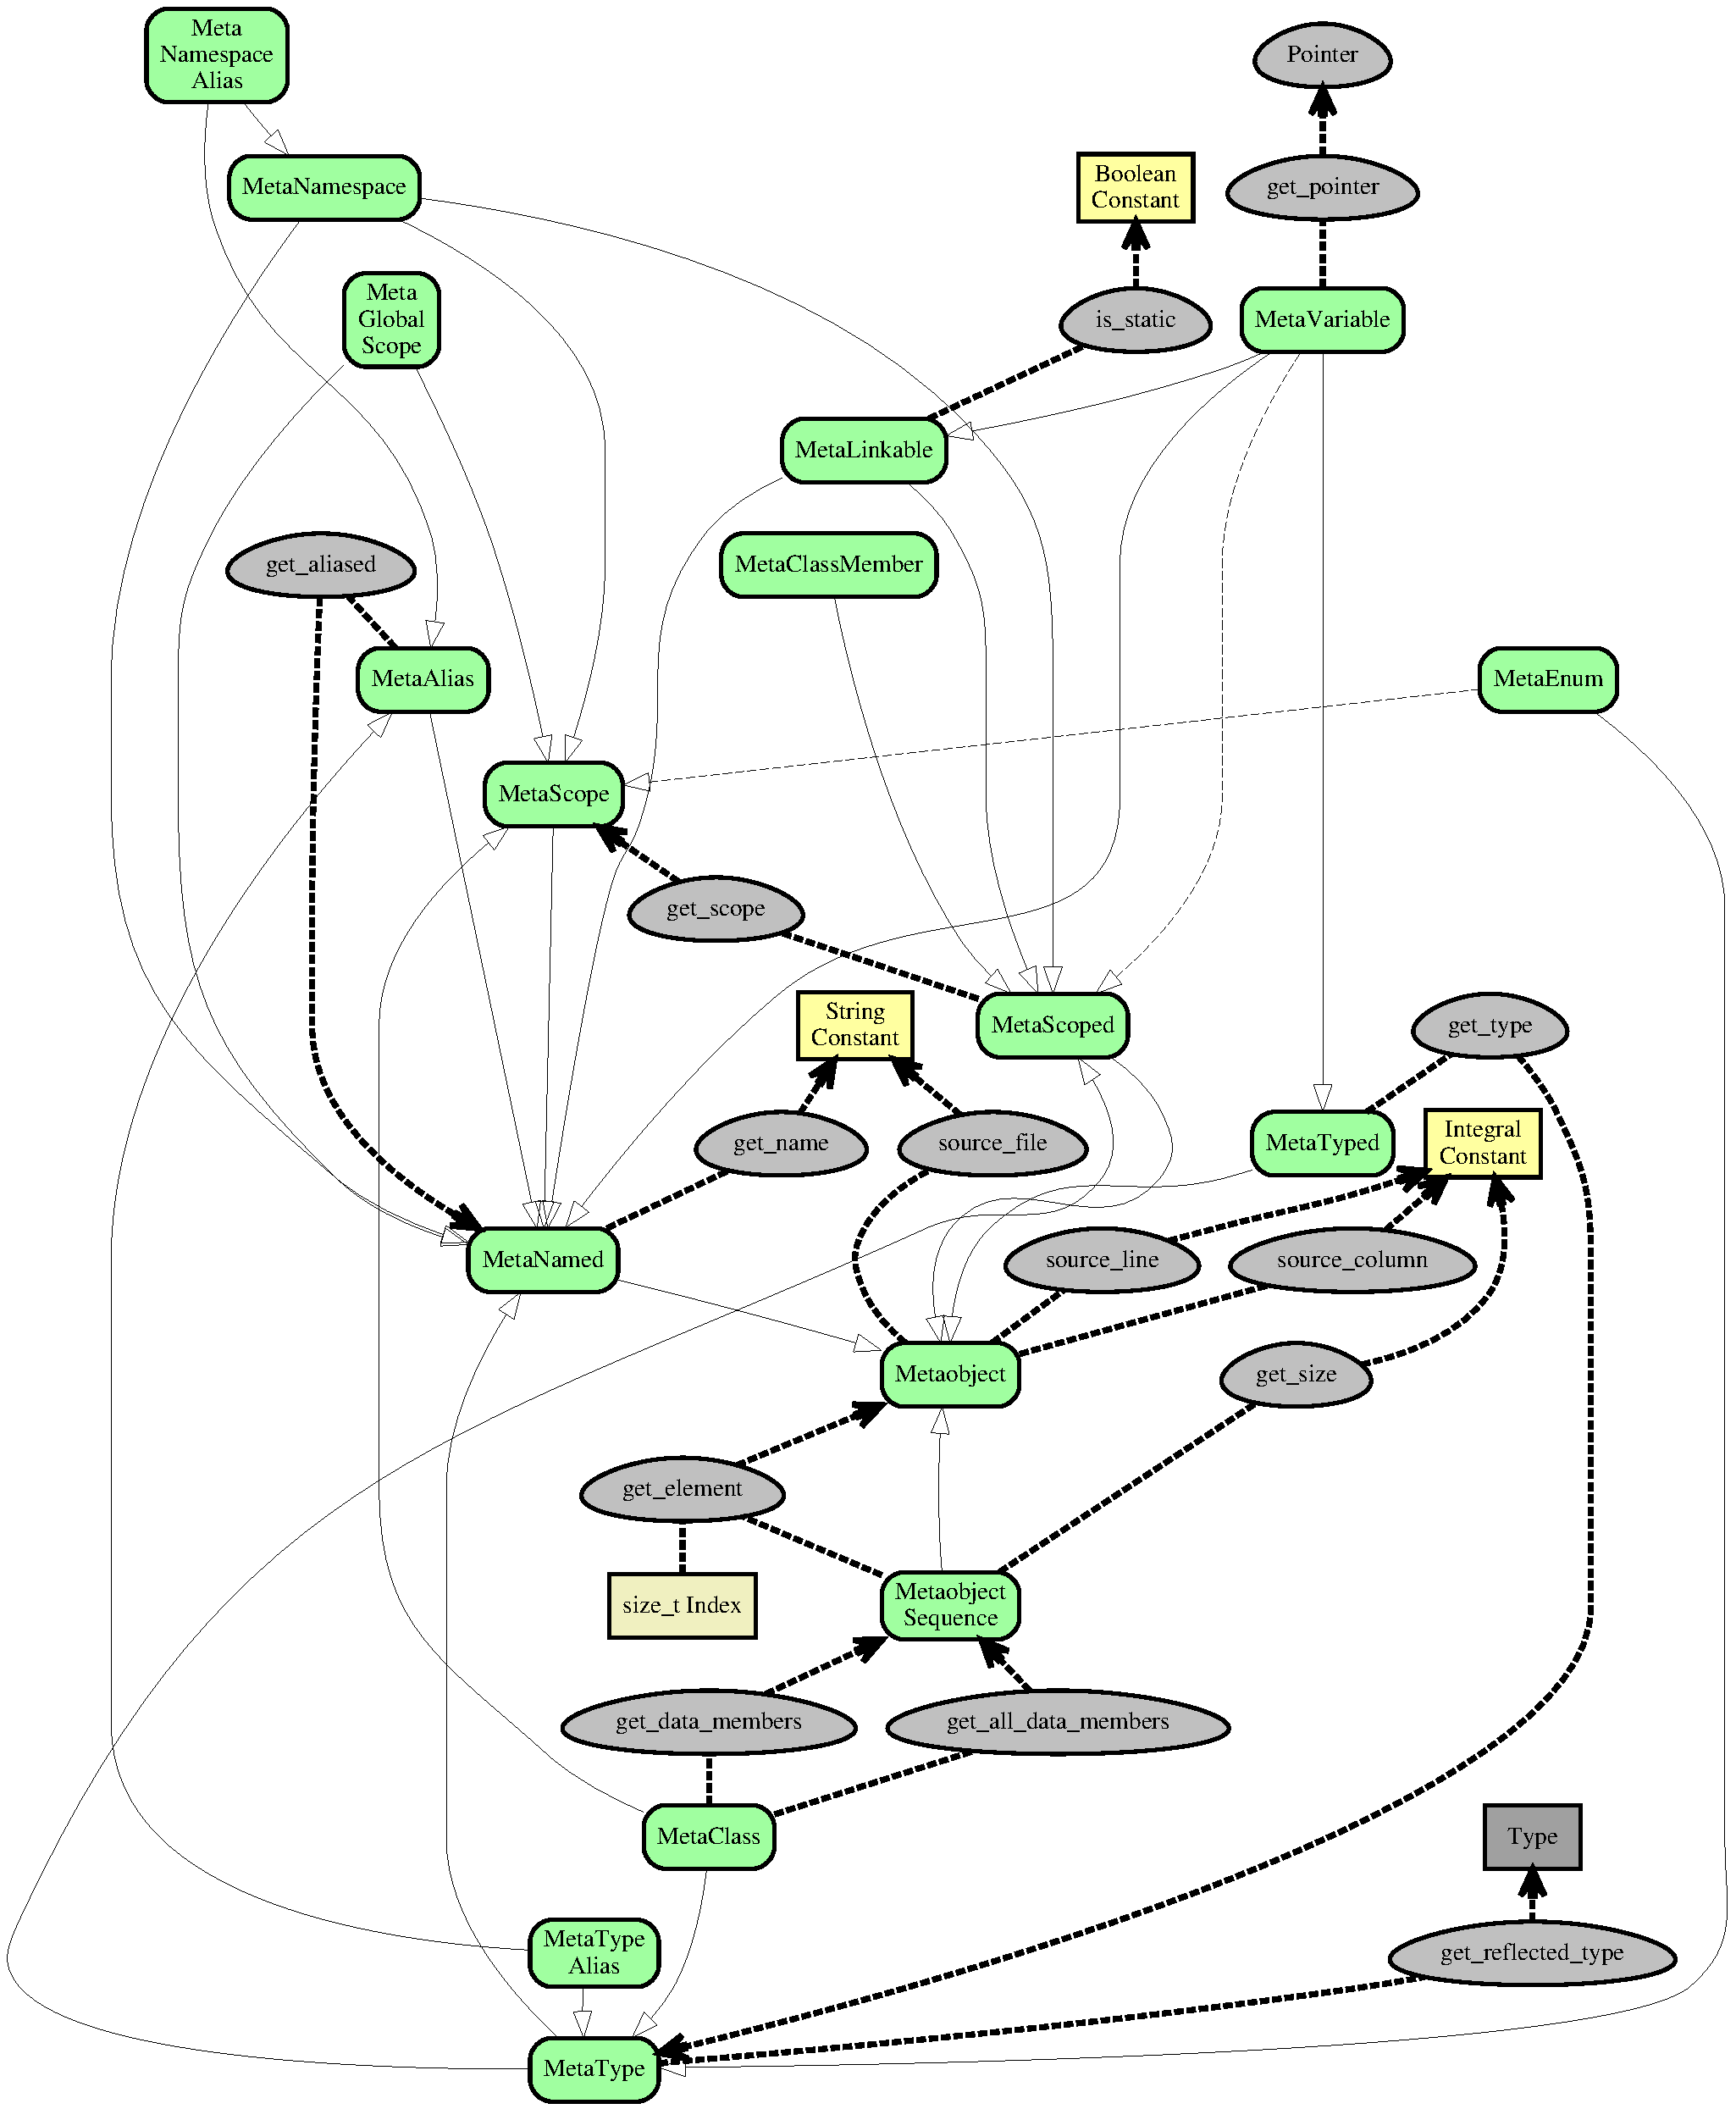
\includegraphics[width=\textwidth]{operations.pdf}
\caption{Metaobject operations}
\end{figure}


\section{Examples}

This section contains multiple examples of usage of the additions proposed above.
The examples assume that the \verb@mirrored@ operator (described above) is used
to obtain the metaobjects and the types, templates, etc. are defined in the
\verb@std::meta@ namespace.

For the sake of brevity

\begin{minted}{cpp}
using namespace std;
\end{minted}

is assumed.

\subsection{Basic traits}

Usage of the \verb@is_metaobject@ trait on non-metaobjects:

\begin{minted}[tabsize=4]{cpp}
static_assert(not(is_metaobject<int>()), "");
static_assert(not(is_metaobject<std::string>()), "");
static_assert(not(is_metaobject<my_class>()), "");
static_assert(not(meta::is_class_member<meta_gs>()), "");
\end{minted}


\subsection{Global scope reflection}

\begin{minted}[tabsize=4]{cpp}
// reflected global scope
typedef mirrored(::) meta_gs;

static_assert(is_metaobject<meta_gs>(), "");

// Is a MetaNamed
static_assert(meta::has_name<meta_gs>(), "");
// Is a MetaScoped
static_assert(meta::has_scope<meta_gs>(), "");
// Is a MetaScope
static_assert(meta::is_scope<meta_gs>(), "");
// Is not a MetaClassMember
static_assert(not(meta::is_class_member<meta_gs>()), "");

// Is a MetaGlobalScope
static_assert(
	is_base_of<
		meta::global_scope_tag,
		meta::category<meta_gs>
	>(), ""
);

// Global scope is its own scope
static_assert(
	is_base_of<
		meta_gs,
		meta::scope<meta_gs>
	>(), ""
);

// Empty base and full name
assert(strlen(meta::base_name<meta_gs>()) == 0);
assert(strcmp(meta::base_name<meta_gs>(), "") == 0);

assert(strlen(meta::full_name<meta_gs>()) == 0);
assert(strcmp(meta::full_name<meta_gs>(), "") == 0);

// the sequence of members
typedef meta::members<meta_gs>::type meta_gs_members;

static_assert(
	meta::size<meta_gs_members>() == 20, // YMMV
	""
);

\end{minted}


\subsection{Namespace reflection}

\begin{minted}[tabsize=4]{cpp}
// reflected namespace std
typedef mirrored(std) meta_std;

static_assert(is_metaobject<meta_std>(), "");

// Is a MetaNamed
static_assert(meta::has_name<meta_std>(), "");
// Is a MetaScoped
static_assert(meta::has_scope<meta_std>(), "");
// Is a MetaScope
static_assert(meta::is_scope<meta_std>(), "");
// Is not a MetaClassMember
static_assert(not(meta::is_class_member<meta_std>()), "");

// Is a MetaNamespace
static_assert(
	is_base_of<
		meta::namespace_tag,
		metaobject_category<meta_std>
	>(), ""
);

// The scope of namespace std is the global scope
static_assert(
	is_base_of<
		meta_gs,
		meta::scope<meta_std>
	>(), ""
);

// The base and full name
assert(strlen(meta::base_name<meta_std>()) == 3);
assert(strcmp(meta::base_name<meta_std>(), "std") == 0);
assert(strlen(meta::full_name<meta_std>()) == 3);
assert(strcmp(meta::full_name<meta_std>(), "std") == 0);
\end{minted}

\subsection{Type reflection}

\begin{minted}[tabsize=4]{cpp}
// reflected type unsigned int
typedef mirrored(unsigned int) meta_uint;

static_assert(is_metaobject<meta_uint>(), "");

// Is a MetaNamed
static_assert(meta::has_name<meta_uint>(), "");
// Is a MetaScoped
static_assert(meta::has_scope<meta_uint>(), "");
// Is not a MetaScope
static_assert(not(meta::is_scope<meta_uint>()), "");
// Is not a MetaClassMember
static_assert(not(meta::is_class_member<meta_uint>()), "");

// Is a MetaType
static_assert(
	is_base_of<
		meta::type_tag,
		meta::category<meta_uint>
	>(), ""
);

// The scope of unsigned int is the global scope
static_assert(
	is_base_of<
		meta_gs,
		meta::scope<meta_uint>
	>(), ""
);

// The original type
static_assert(
	is_same<
		unsigned int,
		meta::original_type<meta_uint>::type
	>(), ""
);

assert(strlen(meta::base_name<meta_uint>()) == 12);
assert(strcmp(meta::base_name<meta_uint>(), "unsigned int") == 0);
assert(strlen(meta::full_name<meta_uint>()) == 12);
assert(strcmp(meta::full_name<meta_uint>(), "unsigned int") == 0);
\end{minted}

\subsection{Typedef reflection}

\begin{minted}[tabsize=4]{cpp}
// reflected typedef std::size_t
typedef mirrored(std::size_t) meta_size_t;

static_assert(is_metaobject<meta_size_t>(), "");

static_assert(meta::has_name<meta_size_t>(), "");
static_assert(meta::has_scope<meta_size_t>(), "");
static_assert(not(meta::is_scope<meta_size_t>()), "");
static_assert(not(meta::is_class_member<meta_size_t>()), "");

// Is a MetaTypedef
static_assert(
	meta::is_alias<meta_size_t>(), ""
);

// The scope of std::size_t is the namespace std
static_assert(
	is_base_of<
		meta_std,
		meta::scope<meta_size_t>
	>(), ""
);

// The original type
static_assert(
	is_same<
		std::size_t,
		meta::original_type<meta_size_t>::type
	>(), ""
);

// the "source" type of the typedef
typedef meta::type<meta_size_t>::type meta_size_t_type;
static_assert(
	is_base_of<
		meta::type_tag,
		meta::category<meta_size_t_type>
	>(), ""
);

// The original type
static_assert(
	is_same<
		std::size_t,
		meta::original_type<meta_size_t_type>::type
	>(), ""
);

assert(strlen(meta::base_name<meta_size_t>()) == 6);
assert(strcmp(meta::base_name<meta_size_t>(), "size_t") == 0);
assert(strlen(meta::full_name<meta_size_t>()) == 11);
assert(strcmp(meta::full_name<meta_size_t>(), "std::size_t") == 0);
// YMMV
assert(strlen(meta::base_name<meta_size_t_type>()) == 12);
assert(strcmp(meta::base_name<meta_size_t_type>(), "unsigned int") == 0);
\end{minted}


\subsection{Class reflection}

\begin{minted}[tabsize=4]{cpp}
struct A
{
	int a;
};

class B
{
private:
	bool b;
public:
	typedef int T;
};

class C
 : public A
 , virtual protected B
{
public:
	static constexpr char c = 'C';

	struct D : A
	{
		static double d;
	} d;
};

union U
{
	long u;
	float v;
};

typedef mirrored(A) meta_A;
typedef mirrored(B) meta_B;
typedef mirrored(C) meta_C;
typedef mirrored(C::D) meta_D;
typedef mirrored(B::T) meta_T;
typedef mirrored(U) meta_U;

// classes are scopes
static_assert(meta::is_scope<meta_A>(), "");
static_assert(meta::is_scope<meta_B>(), "");
static_assert(meta::is_scope<meta_C>(), "");
static_assert(meta::is_scope<meta_D>(), "");
static_assert(meta::is_scope<meta_U>(), "");

// A, B, C, C::D and U are all elaborated types
assert(is_base_of<meta::class_tag, metaobject_category<meta_A>>());
assert(is_base_of<meta::class_tag, metaobject_category<meta_B>>());
assert(is_base_of<meta::class_tag, metaobject_category<meta_C>>());
assert(is_base_of<meta::class_tag, metaobject_category<meta_D>>());
assert(is_base_of<meta::class_tag, metaobject_category<meta_U>>());

static_assert(!meta::is_class_member<meta_A>(), "");
static_assert(!meta::is_class_member<meta_B>(), "");
static_assert(!meta::is_class_member<meta_C>(), "");
static_assert( meta::is_class_member<meta_D>(), "");
static_assert( meta::is_class_member<meta_T>(), "");
static_assert(!meta::is_class_member<meta_U>(), "");

// typenames
assert(strcmp(meta::base_name<meta_A>(), "A") == 0);
assert(strcmp(meta::base_name<meta_B>(), "B") == 0);
assert(strcmp(meta::full_name<meta_D>(), "C::D") == 0);

// reflected elaborated type specifiers for A, B and U
typedef meta::elaborated_type_specifier<meta_A>::type meta_A_ets;
typedef meta::elaborated_type_specifier<meta_B>::type meta_B_ets;
typedef meta::elaborated_type_specifier<meta_U>::type meta_U_ets;

// specifier keywords
assert(strcmp(meta::keyword<meta_A_ets>(), "struct") == 0);
assert(strcmp(meta::keyword<meta_B_ets>(), "class") == 0);
assert(strcmp(meta::keyword<meta_U_ets>(), "union") == 0);

// specifier tags
assert(is_base_of<meta::struct_tag, meta::specifier_category<meta_A_ets>>());
assert(is_base_of< meta::class_tag, meta::specifier_category<meta_B_ets>>());
assert(is_base_of<meta::union_tag, meta::specifier_category<meta_U_ets>>());

// reflected sequences of members of the A,B and C classes
typedef meta::members<meta_A>::type meta_A_members;
typedef meta::members<meta_B>::type meta_B_members;
typedef meta::members<meta_C>::type meta_C_members;

static_assert(meta::size<meta_A_members>() == 1, ""); // A::a
static_assert(meta::size<meta_B_members>() == 2, ""); // B::b,B::T
static_assert(meta::size<meta_C_members>() == 3, ""); // C::c,C::D,C::d

// reflected members of B and C
typedef meta::at<meta_B_members, 0>::type meta_B_b;
typedef meta::at<meta_B_members, 1>::type meta_B_T;
typedef meta::at<meta_C_members, 0>::type meta_C_c;
typedef meta::at<meta_C_members, 1>::type meta_C_D;
typedef meta::at<meta_C_members, 2>::type meta_C_d;

assert(is_base_of<meta::variable_tag, metaobject_category<meta_B_b>>());
assert(is_base_of<meta::typedef_tag, metaobject_category<meta_B_T>>());
assert(is_base_of<meta::class_tag, metaobject_category<meta_C_D>>());

// MetaClassMembers
static_assert( meta::is_class_member<meta_B_b>(), "");
static_assert( meta::is_class_member<meta_B_T>(), "");
static_assert( meta::is_class_member<meta_C_D>(), "");
static_assert( meta::is_class_member<meta_C_d>(), "");

// access specifiers
typedef meta::access_specifier<meta_B_B>::type meta_B_b_access;
typedef meta::access_specifier<meta_C_D>::type meta_C_D_access;

// specifier keywords
assert(strcmp(meta::keyword<meta_B_b_access>(), "private") == 0);
assert(strcmp(meta::keyword<meta_C_D_access>(), "public") == 0);

// sequence of base classes of C
typedef meta::base_classes<meta_C>::type meta_C_bases;

static_assert(meta::size<meta_C_bases>() == 2, ""); // A, B

// MetaInheritances of C->A and C->B
typedef meta::at<meta_C_bases, 0>::type meta_C_base_A;
typedef meta::at<meta_C_bases, 1>::type meta_C_base_B;

// inheritance specifiers
typedef meta::inheritance_specifier<meta_C_base_A>::type meta_C_base_A_it;
typedef meta::inheritance_specifier<meta_C_base_B>::type meta_C_base_B_it;

// access specifiers
typedef meta::access_specifier<meta_C_base_A>::type meta_C_base_A_acc;
typedef meta::access_specifier<meta_C_base_B>::type meta_C_base_B_acc;

// specifier keywords
assert(strcmp(meta::keyword<meta_C_base_A_it>(), "") == 0);
assert(strcmp(meta::keyword<meta_C_base_B_it>(), "virtual") == 0);
assert(strcmp(meta::keyword<meta_C_base_A_acc>(), "public") == 0);
assert(strcmp(meta::keyword<meta_C_base_B_acc>(), "protected") == 0);

// specifier tags
static_assert(
	is_base_of<
		meta::none_tag,
		meta::specifier_category<meta_C_base_A_it>
	>(), ""
);
static_assert(
	is_base_of<
		meta::virtual_tag,
		meta::specifier_category<meta_C_base_B_it>
	>(), ""
);
static_assert(
	is_base_of<
		meta::public_tag,
		meta::specifier_category<meta_C_base_A_acc>
	>(), ""
);

// base classes
static_assert(
	is_base_of<
		meta_A,
		meta::base_class<meta_C_base_A>
	>(), ""
);
static_assert(
	is_base_of<
		meta_B,
		meta::base_class<meta_C_base_B>
	>(), ""
);

\end{minted}


\subsection{Enumeration reflection}

\begin{minted}[tabsize=4]{cpp}
enum E
{
	val_a = 1,
	val_b = 2,
	val_c = 3,
	val_d = 4
};

// reflected enumeration
typedef mirrored(E) meta_E;
// reflected enum values
typedef mirrored(val_a) meta_val_a;
typedef mirrored(val_d) meta_val_d;

// enums are not scopes
static_assert(not(meta::is_scope<meta_E>()), "");
// other traits
static_assert(meta::has_scope<meta_E>(), "");
static_assert(meta::has_name<meta_E>(), "");
static_assert(meta::has_scope<meta_val_a>(), "");
static_assert(meta::has_name<meta_val_a>(), "");

// the categories
assert(is_base_of<meta::enum_tag, metaobject_category<meta_E>>());
assert(is_base_of<meta::constant_tag, metaobject_category<meta_val_a>>());

// names
assert(strcmp(meta::base_name<meta_E>(), "E") == 0);
assert(strcmp(meta::base_name<meta_val_a>(), "val_a") == 0);
assert(strcmp(meta::full_name<meta_val_d>(), "val_d") == 0);

%// reflected elaborated type specifiers for E
%typedef meta::elaborated_type_specifier<meta_E>::type meta_E_ets;

%// specifier keyword
%assert(strcmp(meta::keyword<meta_E_ets>(), "enum") == 0);

%// the members
%typedef meta::members<meta_E>::type meta_E_members;

%assert(meta::size<meta_E_members>() == 4);
%assert(is_base_of<meta_val_a, meta::at<meta_E_members, 0>>());
%assert(is_same<meta_val_d, meta::at<meta_E_members, 3>::type>());

// the scope of the enum values is the same
// as the scope of the enum type
assert(is_same<
	meta::scope<meta_E>::type,
	meta::scope<meta_val_a>::type
>());
assert(is_same<
	meta::scope<meta_E>::type,
	meta::scope<meta::at<meta_E_members, 1>>::type
>());

\end{minted}

\subsection{Strongly-typed enumeration reflection}

\begin{minted}[tabsize=4]{cpp}
enum class E : unsigned short
{
	val_a = 1,
	val_b = 2,
	val_c = 3,
	val_d = 4
};

// reflected enumeration
typedef mirrored(E) meta_E;
// reflected enum values
typedef mirrored(E::val_a) meta_E_val_a;
typedef mirrored(E::val_d) meta_E_val_d;

// enum classes are scopes
static_assert(meta::is_scope<meta_E>(), "");
// other traits
static_assert(meta::has_scope<meta_E>(), "");
static_assert(meta::has_name<meta_E>(), "");
static_assert(meta::has_scope<meta_E_val_a>(), "");
static_assert(meta::has_name<meta_E_val_a>(), "");

// the categories
assert(is_base_of<
	meta::enum_class_tag,
	metaobject_category<meta_E>
>());
assert(is_base_of<
	meta::constant_tag,
	metaobject_category<meta_E_val_a>
>());

// names
assert(strcmp(meta::base_name<meta_E>(), "E") == 0);
assert(strcmp(meta::base_name<meta_E_val_a>(), "val_a") == 0);
assert(strcmp(meta::full_name<meta_E_val_d>(), "E::val_d") == 0);

%// reflected elaborated type specifiers for E
%typedef meta::elaborated_type_specifier<meta_E>::type meta_E_ets;

%// specifier keyword
%assert(strcmp(meta::keyword<meta_E_ets>(), "enum class") == 0);

%// the members
%typedef meta::members<meta_E>::type meta_E_members;

%assert(meta::size<meta_E_members>() == 4);
%assert(is_base_of<meta_E_val_a, meta::at<meta_E_members, 0>>());
%assert(is_same<meta_E_val_d, meta::at<meta_E_members, 3>::type>());

// the scope
assert(is_same<meta_E, meta::scope<meta_E_val_a>::type>());
assert(not(is_same<
	meta::scope<meta_E>::type,
	meta::scope<meta::at<meta_E_members, 1>>::type
>()));
assert(is_same<
	meta::scope<meta_E>::type,
	meta::scope<meta::scope<meta::at<meta_E_members, 1>>>::type
>());

\end{minted}


%TODO



\end{appendices}

\end{document}
